% canon-megatank-reset.tex
% An Open, Native-Linux Reproduction of the Canon MegaTank 5B00 Waste-Ink Reset
% J. Sullivan, 2026
%
% Build: tectonic canon-megatank-reset.tex   (see .github/workflows/build-paper.yml.draft)
% Vendored: IEEEtran.cls, IEEEtran.bst, bytefield.sty, cleveref.sty, balance.sty

\documentclass[conference]{IEEEtran}

\usepackage[utf8]{inputenc}
\usepackage[T1]{fontenc}
\usepackage{amsmath,amssymb}
\usepackage{graphicx}
\usepackage{xcolor}
\usepackage{listings}
\usepackage{booktabs}
\usepackage{array}
\usepackage{tikz}
\usetikzlibrary{arrows.meta,positioning,shapes.geometric,fit,calc,decorations.pathreplacing}
\usepackage{bytefield}
\usepackage{hyperref}
\usepackage{cleveref}   % MUST load after hyperref
\usepackage{balance}
\usepackage{url}
\usepackage{cite}

% ── Colors ──────────────────────────────────────────────────────────────
\definecolor{kwblue}{rgb}{0.0,0.0,0.6}
\definecolor{strred}{rgb}{0.5,0.0,0.0}
\definecolor{cmtgrn}{rgb}{0.25,0.5,0.35}
\definecolor{codebg}{rgb}{0.96,0.96,0.96}
\definecolor{hexhl}{rgb}{0.8,0.0,0.0}

% ── Language defs (Python + Frida-JS), two-tier morekeywords ────────────
\lstdefinelanguage{PyFrida}{
  morekeywords={def,return,if,else,elif,for,while,in,import,from,as,with,
    class,try,except,raise,assert,lambda,yield,not,and,or,is,None,True,False,
    function,const,let,var,new,void},
  morekeywords=[2]{bytes,int,bytearray,bool,str,list,dict,ptr,Process,Memory,
    Interceptor,DeviceIoControl,control_transfer,uint8,uint16,uint32},
  sensitive=true,
  morecomment=[l]{\#},
  morecomment=[l]{//},
  morecomment=[s]{/*}{*/},
  morestring=[b]",
  morestring=[b]',
}

\lstset{
  basicstyle=\footnotesize\ttfamily,
  backgroundcolor=\color{codebg},
  keywordstyle=\color{kwblue}\bfseries,
  keywordstyle=[2]\color{blue!60!black},
  commentstyle=\color{cmtgrn}\itshape,
  stringstyle=\color{strred},
  numbers=left,
  numberstyle=\tiny\color{gray},
  numbersep=5pt,
  frame=single,
  framesep=3pt,
  breaklines=true,
  breakatwhitespace=false,
  showstringspaces=false,
  tabsize=4,
  captionpos=b,
  xleftmargin=1.5em,
  framexleftmargin=1.5em,
  columns=flexible,
  escapeinside={(*@}{@*)},
}

\lstdefinestyle{hex}{
  basicstyle=\footnotesize\ttfamily,
  backgroundcolor=\color{codebg},
  numbers=none,
  frame=single,
  framesep=3pt,
  breaklines=true,
  xleftmargin=1em,
  framexleftmargin=1em,
}

\lstdefinestyle{shell}{
  basicstyle=\footnotesize\ttfamily,
  backgroundcolor=\color{codebg},
  numbers=none,
  frame=single,
  framesep=3pt,
  breaklines=true,
  xleftmargin=1em,
  framexleftmargin=1em,
  morekeywords={sudo,lsusb,tshark,modprobe,frida,tectonic,canon-megatank,
    dumpcap,echo,ipptool},
  keywordstyle=\color{kwblue}\bfseries,
}

% ════════════════════════════════════════════════════════════════════════
\begin{document}

\title{An Open, Native-Linux Reproduction of the Canon MegaTank
5B00 Waste-Ink Reset: Reverse Engineering the usbprint Vendor Transport
and the Session-Keyword Write Cipher}

\author{\IEEEauthorblockN{J. Sullivan}
\IEEEauthorblockA{2026}}

\maketitle

% ════════════════════════════════════════════════════════════════════════
\begin{abstract}
Canon MegaTank (G-series) inkjet printers permanently disable themselves
with support code 5B00 once an internal waste-ink absorber counter
saturates, reporting only ``service is required'' with no user-accessible
reset. On the G5000/G6000/G7000 generation the classic service-mode clear
is disabled in firmware, so the only working remedy is a commercial,
cloud-gated Windows tool that validates a single-use, per-printer key
against a vendor server. We present a fully open, native-Linux,
key-free, and cloud-free reproduction of that reset, derived through a
trace$\leftrightarrow$decompile$\leftrightarrow$correlate methodology:
host \texttt{usbmon} wire capture, Frida instrumentation of the Windows
tool inside a virtual machine, and Ghidra decompilation of both the
vendor tool and Windows' \texttt{usbprint.sys}. We recover the transport
(a USB \emph{vendor} control transfer, \texttt{0x41} OUT / \texttt{0xC1}
IN, with \texttt{bRequest} carrying the command byte), the session
protocol (a plain \texttt{set\_session}, a live per-session device
keyword read via \texttt{get\_keyword}, and an enciphered
\texttt{set\_command} write), and the write cipher itself---a functor
envelope whose buffer roles are swapped relative to the naive reading,
validated byte-exact (23/23) against a genuine captured frame. To obtain
that ground-truth frame we bypass the tool's three cloud-licensing gates
with a one-byte-per-gate \texttt{JZ}$\rightarrow$\texttt{JMP} patch, and
we prove by decompilation that no cloud byte ever reaches the reset
payload, keyword, or completion: the cloud is licensing only. The
resulting native tool clears 5B00 on real hardware (Canon device
\texttt{04a9:1865}/service \texttt{04a9:12fe}) using only libusb and one
live keyword read, behind a stack of safety gates (test-unit isolation,
EEPROM dump, write budget, lockfile). We additionally document an
operationally critical nuance: the cleared counter commits only on a
clean power-button shutdown (printhead-park EEPROM flush), not on an
abrupt unplug.
\end{abstract}

\begin{IEEEkeywords}
Canon MegaTank, waste-ink reset, 5B00, USB reverse engineering, usbprint
vendor control transfer, session-keyword cipher, DRM bypass, Frida,
Ghidra, right to repair
\end{IEEEkeywords}

% ════════════════════════════════════════════════════════════════════════
\section{Introduction}
\label{sec:intro}

Canon MegaTank printers route stray ink---from cleaning cycles, borderless
printing, and power-on priming---into an internal absorber pad. Firmware
maintains a software counter that estimates absorber saturation, and when
that counter crosses a threshold the printer halts with support code 5B00
and the message ``service is required.'' Canon offers no user reset;
official guidance is warranty replacement or disposal~\cite{canon-5b00-support}.
On earlier PIXMA models a panel key combination cleared the counter, but
on the G5000/G6000/G7000 generation that built-in reset is removed in
firmware: the printer still \emph{enters} service mode, but accepts and
silently ignores the legacy clear command.

In practice the only path back to a working printer on this generation is
a commercial Windows utility (WICReset / Printer Potty) that requires a
single-use, per-printer key validated online against a vendor
server~\cite{octoinkjet-wicreset}. This is the canonical
software-counter-as-DRM situation: a mechanically serviceable device is
bricked by a counter, and the unlock is gated behind a proprietary,
network-dependent, paid tool. Replacing or externally plumbing the
physical absorber is straightforward; clearing the firmware counter is
the hard part.

\textbf{Our contribution} is an open, native-Linux, key-free, and
cloud-free reproduction of the MegaTank 5B00 reset, together with the
reverse-engineering evidence that makes it reproducible. Specifically:

\begin{enumerate}
\item We recover the service-mode \emph{transport} by decompiling
  Windows' \texttt{usbprint.sys}: the maintenance commands are USB
  \emph{vendor} control transfers, not bulk transfers
  (\Cref{sec:transport}).
\item We document the session \emph{protocol}---plain
  \texttt{set\_session}, a live per-session device keyword from
  \texttt{get\_keyword}, and the enciphered \texttt{set\_command}
  writes---and characterize the empty \texttt{get\_command} completion
  (\Cref{sec:protocol}).
\item We crack the write \emph{cipher}: a functor envelope whose buffer
  roles (subject vs.\ seed) are swapped relative to the obvious reading,
  validated 23/23 against a genuine captured frame (\Cref{sec:cipher}).
\item We obtain that genuine frame by bypassing three cloud-licensing
  gates and \emph{prove by decompilation} that the reset is
  cloud-independent (\Cref{sec:drm}).
\item We reproduce the reset natively on real hardware and document the
  power-button commit nuance (\Cref{sec:native}), behind a safety-gate
  stack (\Cref{sec:safety}) with hardware results (\Cref{sec:results}).
\end{enumerate}

All findings, scripts, and the reference codec are open source under a
clean-room, interoperability, and right-to-repair framing
(\Cref{sec:r2r,sec:artifact})~\cite{canon-megatank-reset}.

% ════════════════════════════════════════════════════════════════════════
\section{Background}
\label{sec:background}

\subsection{Canon MegaTank service mode}
\label{sec:bg-servicemode}

A MegaTank printer enumerates differently depending on mode. In normal
operation the G6020 is USB device \texttt{04a9:1865} with several
interfaces. Entering service mode (a panel power/resume key sequence)
re-enumerates the printer as \texttt{04a9:12fe}: a single printer-class
interface (interface~0, alternate~0) whose IEEE-1284 device ID advertises
\texttt{MFG:Canon;CMD:BJL,\ldots;PSE:KMDA10021}. Maintenance commands are
issued over this service-mode interface. Crucially, on this generation the
firmware accepts the legacy clear and does nothing with it---the gate is
not a different opcode but a refusal to honor an unauthenticated write
(\Cref{sec:problem}).

\subsection{The pixma firmware lineage}
\label{sec:bg-pixma}

Open Canon reverse engineering descends from the Context IS ``doomed
encryption'' work on PIXMA firmware updates~\cite{contextis-canon} and the
\texttt{leecher1337/pixma} toolkit~\cite{leecher-pixma}, which recovers a
firmware XOR key from a known SREC plaintext and unpacks a Thumb-compressed
payload. That lineage is a \emph{firmware-unpack} toolkit: it contains no
service-mode, USB-framing, or waste-counter logic, and ships without a
license. The SANE \texttt{pixma} scanner backend~\cite{sane-pixma} shows
Canon's command-framing style but operates on a bulk channel unrelated to
the maintenance transport. The open Epson lineage is more directly
transferable in spirit: tools such as \texttt{reink}~\cite{reink-elena},
\texttt{epson\_print\_conf}~\cite{ircama-epson-print-conf}, and
\texttt{epson-printer-snmp}~\cite{zedeldi-epson-snmp} reset Epson
maintenance counters, the last by sniffing WICReset---the same
capture-and-correlate method we apply to Canon. No open Canon G-series
equivalent existed prior to this work.

\subsection{usbprint vendor control transfers}
\label{sec:bg-usbprint}

Windows binds the service-mode interface to the \texttt{usbprint.sys}
printer minidriver, which exposes private IOCTLs. Two are load-bearing
here: \texttt{IOCTL\_USBPRINT\_VENDOR\_SET\_COMMAND} (\texttt{0x220038})
and \texttt{VENDOR\_GET\_COMMAND} (\texttt{0x22003c}). As we show in
\Cref{sec:transport}, each maps to a single USB \emph{vendor}-class,
interface-recipient control transfer on endpoint~0---not to a bulk
transfer on the printer's data endpoints. This distinction is the reason
every prior native attempt stalled.

% ════════════════════════════════════════════════════════════════════════
\section{Problem Analysis}
\label{sec:problem}

\subsection{Symptom characterization}
\label{sec:problem-symptom}

The printer reports 5B00 and refuses to print. Over IPP the printer-state
is \texttt{stopped} with a \texttt{marker-waste-ink-receptacle-full}
alert:

\begin{lstlisting}[style=shell,caption={5B00 surfaces as an IPP printer-state
alert.},label={lst:ipp-stopped}]
$ ipptool -tv ipp://printer/ get-attrs.test
  printer-state = stopped (5)
  printer-state-reasons = marker-waste-ink-receptacle-full
\end{lstlisting}

The legacy service-mode clear is accepted on the wire but does not
persist. \Cref{lst:legacy-clear} shows the falsified attempt: a
well-formed vendor control-OUT carrying the old payload returns an ACK,
yet 5B00 survives a power cycle.

\begin{lstlisting}[style=shell,caption={Legacy clear is ACKed but does not
clear 5B00 (falsified, multiple sessions).},label={lst:legacy-clear}]
# vendor control-OUT, legacy payload  ->  device ACK 5
ctrl(0x40, 0x85, 0x0000, 0x0000, [00 03 01 03 07])
# power-cycle  ->  printer-state still "stopped", 5B00 returns
\end{lstlisting}

\subsection{The firmware authorization barrier}
\label{sec:problem-barrier}

\Cref{tab:barrier} summarizes the falsification campaign. The pattern is
consistent: every unauthenticated frame---over bulk or control, with the
checkbox flag set or not, with the index in the payload or in
\texttt{wValue}---is accepted (ACK) but ignored (5B00 persists). The
working commercial tool differs not in the opcode but in opening an
authenticated \emph{session} keyed to a live device value before writing.

\begin{table}[ht]
\centering
\caption{Falsified Reset Attempts (G6020, service mode \texttt{12fe})}
\label{tab:barrier}
\begin{tabular}{@{}lll@{}}
\toprule
Attempt & Channel & Outcome \\
\midrule
Bare \texttt{85\,00\,00\,00\,03\,01\,03\,07} & bulk OUT \texttt{0x01} & ACK; 5B00 persists \\
Legacy payload, flag \texttt{0x81} & vendor ctrl-OUT & ACK 5; 5B00 persists \\
Index in \texttt{wValue} & vendor ctrl-OUT & ACK; 5B00 persists \\
Plain \texttt{set\_session 0x81} & vendor ctrl-OUT & STALL \\
Bulk-IN read \texttt{0x82} & bulk IN & ZLP (0 bytes) \\
\midrule
\multicolumn{3}{l}{\footnotesize Authenticated session
(\Cref{sec:protocol}) is the only path that clears.} \\
\bottomrule
\end{tabular}
\end{table}

% ════════════════════════════════════════════════════════════════════════
\section{Method: The Trace--Decompile--Correlate Trifecta}
\label{sec:method}

Our methodology triangulates three independent evidence sources so that
each closes the others' blind spots (\Cref{fig:trifecta}). \emph{Trace}:
host \texttt{usbmon} captures the literal wire URBs at the bus, which a
TLS-encrypted in-process view cannot fake. \emph{Decompile}: Ghidra
recovers the intended semantics---the IOCTL$\rightarrow$URB mapping in
\texttt{usbprint.sys} and the frame builder/cipher in the vendor tool---which
opaque ciphertext on the wire cannot reveal. \emph{Correlate}: Frida hooks
\texttt{DeviceIoControl} inside the tool to expose plaintext in/out buffers
with timestamps, pairing each decompiled routine to the exact URB it
produced. The phases below are executed within one VM session against one
genuine reset so the three layers describe the \emph{same} event.

\begin{figure}[ht]
\centering
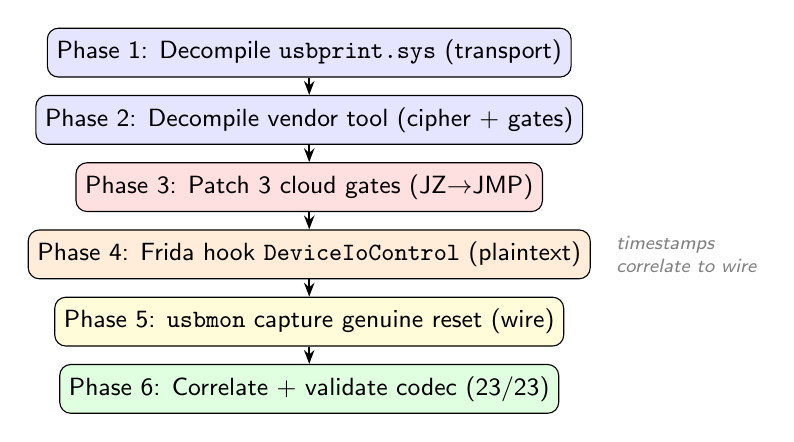
\begin{tikzpicture}[
  phase/.style={draw, rounded corners, minimum width=5.2cm,
    minimum height=0.62cm, font=\small\sffamily, align=center},
  arr/.style={-{Stealth[length=5pt]}, thick},
  note/.style={font=\scriptsize\sffamily\itshape, text=gray, align=left},
]
  \node[phase, fill=blue!10]   (p1) at (0,0)
    {Phase 1: Decompile \texttt{usbprint.sys} (transport)};
  \node[phase, fill=blue!10, below=0.22cm of p1] (p2)
    {Phase 2: Decompile vendor tool (cipher + gates)};
  \node[phase, fill=red!12,  below=0.22cm of p2] (p3)
    {Phase 3: Patch 3 cloud gates (JZ$\rightarrow$JMP)};
  \node[phase, fill=orange!15, below=0.22cm of p3] (p4)
    {Phase 4: Frida hook \texttt{DeviceIoControl} (plaintext)};
  \node[phase, fill=yellow!15, below=0.22cm of p4] (p5)
    {Phase 5: \texttt{usbmon} capture genuine reset (wire)};
  \node[phase, fill=green!12, below=0.22cm of p5] (p6)
    {Phase 6: Correlate + validate codec (23/23)};

  \draw[arr] (p1) -- (p2);
  \draw[arr] (p2) -- (p3);
  \draw[arr] (p3) -- (p4);
  \draw[arr] (p4) -- (p5);
  \draw[arr] (p5) -- (p6);

  \node[note, right=0.2cm of p4] {timestamps\\correlate to wire};
\end{tikzpicture}
\caption{The trace$\leftrightarrow$decompile$\leftrightarrow$correlate
trifecta. Phases 1--2 recover intended semantics; phases 3--5 capture one
genuine reset at the IOCTL and wire layers simultaneously; phase 6 proves
the native codec reproduces the captured frame byte-exact.}
\label{fig:trifecta}
\end{figure}

The capture environment is a Win11 guest with the printer passed through
via QEMU USB passthrough; per prior lab notes the guest requires an
e1000e NIC and NTLM WinRM transport for reliable automation. We treat the
VM as equivalent to bare metal for capture purposes: the device sits on the
real bus and the wire bytes are identical.

% ════════════════════════════════════════════════════════════════════════
\section{Transport Reverse Engineering}
\label{sec:transport}

We decompiled \texttt{usbprint.sys} (Win11 24H2,
\texttt{10.0.26100.8328}) and traced the device-control dispatch to the
\texttt{VENDOR\_SET}/\texttt{VENDOR\_GET} handlers. Both allocate a
\texttt{\_URB\_CONTROL\_VENDOR\_OR\_CLASS\_REQUEST} (function
\texttt{0x0018}, \texttt{URB\_FUNCTION\_VENDOR\_INTERFACE}) and submit it
to the bus driver---there is no bulk path. The handler reads the IOCTL
input buffer and assigns the URB fields as follows: \texttt{bRequest =
inBuf[0]}; \texttt{wValue = (inBuf[1] << 8) | inBuf[2]}; \texttt{wIndex =
(bInterfaceNumber << 8) | bAlternateSetting}; and---decisively---the
\emph{entire} input buffer becomes the data stage
(\texttt{TransferBuffer = SystemBuffer}, \texttt{TransferBufferLength =
InputBufferLength}). The driver does \emph{not} strip the three header
bytes: \texttt{inBuf[0]} seeds \texttt{bRequest} \emph{and} remains the
first data byte.

\Cref{fig:vendor-frame} shows the resulting on-wire control frame.
\texttt{VENDOR\_SET} yields \texttt{bmRequestType = 0x41} (vendor,
interface, host$\rightarrow$device); \texttt{VENDOR\_GET} yields
\texttt{0xC1} (vendor, interface, IN). This was cross-checked against two
mappings the live device already confirmed: \texttt{GET\_1284\_ID}
(class/interface/IN $\Rightarrow$ \texttt{0xA1}) and \texttt{VENDOR\_GET}
of the firmware version (\texttt{0xC1/0x8a}), both byte-exact.

\begin{figure}[ht]
\centering
\begin{bytefield}[bitwidth=1.8em]{8}
\bitheader{0-7} \\
\bitbox{8}{\texttt{bmRequestType}: \texttt{0x41} OUT / \texttt{0xC1} IN} \\
\bitbox{8}{\texttt{bRequest} = \texttt{inBuf[0]} (command byte)} \\
\bitbox{4}{\texttt{wValue} hi = \texttt{inBuf[1]}}
\bitbox{4}{\texttt{wValue} lo = \texttt{inBuf[2]}} \\
\bitbox{4}{\texttt{wIndex} = iface}
\bitbox{4}{(\texttt{0x0000})} \\
\bitbox{8}{\texttt{wLength} = full frame length} \\
\bitbox{8}{Data stage: the ENTIRE frame, verbatim} \\
\end{bytefield}
\caption{usbprint vendor control frame. The command byte and argument
bytes seed the setup packet \emph{and} remain at the head of the data
stage---the driver never strips \texttt{inBuf[0..2]}. Splitting the header
off the data stage was the cause of every prior control-pipe STALL.}
\label{fig:vendor-frame}
\end{figure}

The endianness of \texttt{wValue} is explicit in the decompile
(\texttt{inBuf[1]} is the high byte); all target frames carry argument
bytes \texttt{00 00}, so \texttt{wValue = 0x0000} regardless, but a future
non-zero argument must follow the decompiled order. The native transport
is a thin libusb wrapper: \texttt{send\_command} issues a
\texttt{0x41} control-OUT with the whole frame as data;
\texttt{send\_and\_receive} issues a \texttt{0xC1} control-IN for a bare
3-byte read header and the read length as \texttt{wLength}
(\Cref{sec:protocol}).

% ════════════════════════════════════════════════════════════════════════
\section{The Wire Protocol and the Per-Session Keyword}
\label{sec:protocol}

The reset is an ordered session of four logical commands over the vendor
transport (\Cref{fig:statemachine}). The command byte rides in
\texttt{bRequest}: \texttt{0x81} \texttt{set\_session}, \texttt{0x82}
\texttt{get\_keyword}, \texttt{0x85} \texttt{set\_command}, \texttt{0x86}
\texttt{get\_command}.

\begin{figure}[ht]
\centering
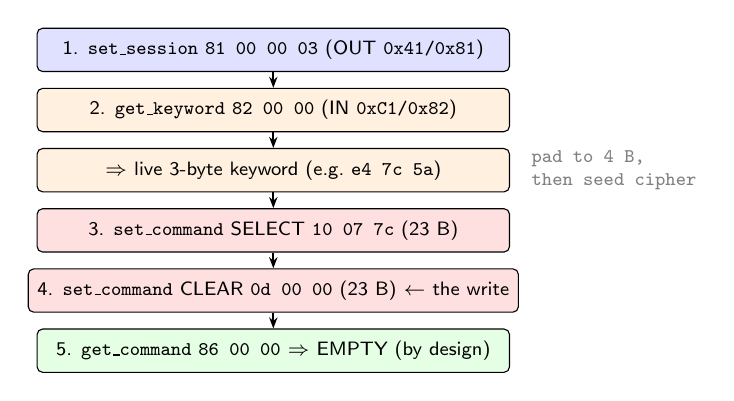
\begin{tikzpicture}[
  stepbox/.style={draw, rounded corners=2pt, minimum width=6.0cm,
    minimum height=0.55cm, font=\scriptsize\sffamily, align=center},
  arr/.style={-{Stealth[length=4pt]}, thick},
  reg/.style={font=\scriptsize\ttfamily, text=gray, align=left},
]
  \node[stepbox, fill=blue!12]   (s1) at (0,0)
    {1. \texttt{set\_session} \texttt{81 00 00 03} (OUT \texttt{0x41/0x81})};
  \node[stepbox, fill=orange!12, below=0.2cm of s1] (s2)
    {2. \texttt{get\_keyword} \texttt{82 00 00} (IN \texttt{0xC1/0x82})};
  \node[stepbox, fill=orange!12, below=0.2cm of s2] (s3)
    {$\Rightarrow$ live 3-byte keyword (e.g.\ \texttt{e4 7c 5a})};
  \node[stepbox, fill=red!12,    below=0.2cm of s3] (s4)
    {3. \texttt{set\_command} SELECT \texttt{10 07 7c} (23 B)};
  \node[stepbox, fill=red!12,    below=0.2cm of s4] (s5)
    {4. \texttt{set\_command} CLEAR \texttt{0d 00 00} (23 B) $\leftarrow$ the write};
  \node[stepbox, fill=green!10,  below=0.2cm of s5] (s6)
    {5. \texttt{get\_command} \texttt{86 00 00} $\Rightarrow$ EMPTY (by design)};

  \draw[arr] (s1) -- (s2);
  \draw[arr] (s2) -- (s3);
  \draw[arr] (s3) -- (s4);
  \draw[arr] (s4) -- (s5);
  \draw[arr] (s5) -- (s6);

  \node[reg, right=0.15cm of s3, align=left]
    {pad to 4 B,\\then seed cipher};
\end{tikzpicture}
\caption{The service-mode reset state machine. The live keyword from
step~2 is the only runtime input; it keys the two enciphered
\texttt{set\_command} writes to the session. The \texttt{get\_command}
read-back is empty on this device and must not be used as a success gate.}
\label{fig:statemachine}
\end{figure}

\noindent\textbf{The live keyword.} \texttt{get\_keyword} returns a
3-byte per-session value (e.g.\ \texttt{e4 7c 5a}). The cipher seed is
4~bytes, so the reply is right-padded to \texttt{e4 7c 5a 00} before
seeding the encoder. This read \emph{must} precede the writes: it binds
them to the live session. We observed (and reproduced) that a
\texttt{get\_version} prime \texttt{8a 00 00} returns a 20-byte enciphered
reply that decrypts locally to the model string ``Canon G6000 series''
with zero cloud interaction---direct corroboration that the device, not
the cloud, sources session state.

\noindent\textbf{The empty completion.} \texttt{get\_command}
(\texttt{86 00 00}) returns an empty reply on this device, and there is no
finalize command. Code that gates success on a non-empty \texttt{0x86}
read will wrongly fail a successful reset; the clear is committed by the
two writes plus a clean power-off (\Cref{sec:native}), not by
\texttt{0x86}.

% ════════════════════════════════════════════════════════════════════════
\section{The Write Cipher}
\label{sec:cipher}

\subsection{Frame shape}
\label{sec:cipher-shape}

A genuine \texttt{set\_command} is a single 23-byte frame: the 3-byte
header \texttt{85 00 00} followed by a 20-byte ciphertext
(\Cref{fig:envelope}). It is \emph{not} a select/clear pair, and not the
naive ``header $\parallel$ 4-byte enciphered keyword'' shape that an early
model emitted. The genuine captured payload for the SELECT operand is
\texttt{db bb 00 67 59 a1 b0 1f 84 2f d5 83 04 4a 3a c3 51 d2 b1 ef}:
20 distinct, high-entropy bytes, exactly one zero, with no \texttt{00 12
01} envelope marker visible on the wire.

\begin{figure}[ht]
\centering
\begin{bytefield}[bitwidth=1.55em]{10}
\bitheader{0-9} \\
\bitbox{3}{\texttt{85 00 00}\\(header)}
\bitbox{7}{20-byte ciphertext (payload), bytes 0--6} \\
\wordbox{1}{\ldots payload bytes 7--16 \ldots} \\
\bitbox{3}{payload\\17--19}
\bitbox{7}{wire = 23 bytes total} \\
\end{bytefield}
\caption{The 23-byte \texttt{set\_command} frame: header
\texttt{85 00 00} $\parallel$ 20-byte enciphered payload. The whole frame
is the control-OUT data stage; the header must never be split from the
payload.}
\label{fig:envelope}
\end{figure}

\subsection{The functor buffer-role swap}
\label{sec:cipher-functor}

The cipher is built from two functors recovered from the vendor tool's
decompile. A functor-3 step deterministically expands the application
command into a 20-byte \emph{envelope}; a functor-2 step then transforms
that envelope under a 4-byte \emph{bound keyword}. The non-obvious
correction---the crux of the crack---is that the buffer roles are swapped
relative to the naive reading: the 20-byte envelope is the
\textsc{subject} of functor-2 and the bound keyword is the \textsc{seed},
not the reverse. \Cref{lst:cipher} states the validated construction.

\begin{lstlisting}[language=PyFrida,caption={The validated CANON-SR5 write
construction (functor-3 envelope, functor-2 keyword bind, role-swapped).},
label={lst:cipher}]
app      = b"\x85\x00\x00" + operand        # e.g. 10 07 7c  (SELECT)
envelope = envelope3(method=3, app)         # 20-byte envelope
bound    = bind_keyword(method, kw_pad4)    # 4-byte session bind
# SUBJECT = envelope (20B), SEED = bound keyword (4B):
payload  = functor2(method, envelope,
                    seed=bound, send=True)   # 20 bytes
wire     = b"\x85\x00\x00" + payload         # 23 bytes
\end{lstlisting}

\subsection{23/23 validation}
\label{sec:cipher-valid}

For the genuine captured live keyword \texttt{e4 7c 5a} (padded
\texttt{e4 7c 5a 00}, bound \texttt{00 35 a9 09}), both independent code
paths---a parser-driven encoder loaded from the recovered template and a
from-scratch reimplementation of the decompiled transform---reproduce the
captured wire frames byte-exact (\Cref{lst:2323}). This is the central
positive result: 23/23 bytes per frame, on the genuine session keyword,
from two non-shared implementations.

\begin{lstlisting}[style=hex,caption={Byte-exact (23/23) reproduction of
the genuine captured frames for keyword \texttt{e4 7c 5a}.},label={lst:2323}]
SELECT set_command 10 07 7c
 850000 dbbb006759a1b01f842fd583044a3ac351d2b1ef
CLEAR  set_command 0d 00 00   <- the 5B00 write
 850000 4dbb006759a1b01f842fd58319a83a627bafb1ef
\end{lstlisting}

We also report a deliberate \emph{negative} result. The keyword reply is
3~bytes but the seed is 4~bytes, and the correct 4th-byte padding rule
cannot be inferred from a single \texttt{(keyword, payload)} pair: the
payload is a full-entropy, operand- and keyword-dependent ciphertext, and
one sample cannot separate the keyword keystream from the operand
dependence. The cipher reproduces the captured frame exactly and is
keyword-parametric (it also reproduces a differently-keyed prior capture),
but generalizing the padding rule to arbitrary keywords requires a
controlled multi-sample campaign, analogous to the $\sim$40-sample
campaign that cracked the read-side codec. We state this boundary
explicitly rather than overclaim.

% ════════════════════════════════════════════════════════════════════════
\section{DRM Bypass for Ground Truth, and the Cloud-Independence Proof}
\label{sec:drm}

\subsection{Three cloud gates}
\label{sec:drm-gates}

To capture a genuine frame we had to run the commercial tool to the point
of emitting the reset, which requires passing its online licensing. The
reset orchestrator (\texttt{Core::ActionCanonDeviceClearCounters}) reaches
the net-free emit routine (\texttt{clearCounters}) only through three
cloud round-trips, each guarded by a conditional jump
(\Cref{fig:gates}): \texttt{RESET\_GUID}, then \texttt{QUERY\_KEYS}
transport-success, then a \texttt{QUERY\_KEYS} validity bit. In an offline
VM all three stall on the licensing socket, and the tool aborts before any
USB write.

\begin{figure}[ht]
\centering
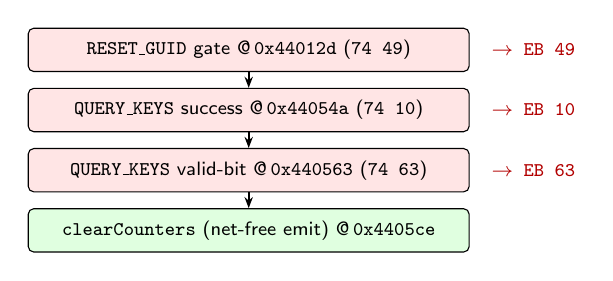
\begin{tikzpicture}[
  gate/.style={draw, rounded corners=2pt, minimum width=5.6cm,
    minimum height=0.55cm, font=\scriptsize\sffamily, align=center},
  arr/.style={-{Stealth[length=4pt]}, thick},
  patch/.style={font=\scriptsize\ttfamily, text=red!70!black, align=left},
]
  \node[gate, fill=red!10]   (g0) at (0,0)
    {\texttt{RESET\_GUID} gate @\,\texttt{0x44012d} (\texttt{74 49})};
  \node[gate, fill=red!10, below=0.2cm of g0] (g1)
    {\texttt{QUERY\_KEYS} success @\,\texttt{0x44054a} (\texttt{74 10})};
  \node[gate, fill=red!10, below=0.2cm of g1] (g2)
    {\texttt{QUERY\_KEYS} valid-bit @\,\texttt{0x440563} (\texttt{74 63})};
  \node[gate, fill=green!12, below=0.2cm of g2] (em)
    {\texttt{clearCounters} (net-free emit) @\,\texttt{0x4405ce}};

  \draw[arr] (g0) -- (g1);
  \draw[arr] (g1) -- (g2);
  \draw[arr] (g2) -- (em);

  \node[patch, right=0.15cm of g0] {$\rightarrow$ \texttt{EB 49}};
  \node[patch, right=0.15cm of g1] {$\rightarrow$ \texttt{EB 10}};
  \node[patch, right=0.15cm of g2] {$\rightarrow$ \texttt{EB 63}};
\end{tikzpicture}
\caption{The three cloud-licensing gates on the path to the net-free
emit. Each is forced taken by rewriting the conditional jump
\texttt{JZ}\,(\texttt{0x74}) to an unconditional \texttt{JMP}\,(\texttt{0xEB}),
preserving the displacement byte so the target is unchanged. Patching only
the two \texttt{QUERY\_KEYS} gates is insufficient: \texttt{RESET\_GUID}
runs first and stalls the same way.}
\label{fig:gates}
\end{figure}

The patch is one byte per gate (\Cref{lst:frida}), applied at spawn via
Frida so it is in place before the Reset button is clicked. Each rewrite
keeps the relative displacement, so the unconditional jump lands on the
same target the original would on success. A guard aborts loudly if the
opcode is not \texttt{0x74}, since the offsets are exact only for this
binary hash; the image is ASLR-enabled, so a runtime slide is computed.

\begin{lstlisting}[language=PyFrida,caption={Forcing a licensing gate
taken: \texttt{JZ}$\rightarrow$\texttt{JMP} (\texttt{0x74}$\rightarrow$\texttt{0xEB}),
displacement preserved.},label={lst:frida}]
function jzToJmp(addr) {
  const p = va(addr);                 // static VA + ASLR slide
  if (p.readU8() !== 0x74) {          // guard: hash-specific offsets
    console.log("[!] expected 0x74 -- ABORT"); return;
  }
  Memory.patchCode(p, 1, code =>      // W^X-safe, flushes i-cache
    code.writeU8(0xEB));
}
jzToJmp("0x44012d");  // RESET_GUID
jzToJmp("0x44054a");  // QUERY_KEYS success
jzToJmp("0x440563");  // QUERY_KEYS valid-bit
\end{lstlisting}

\subsection{No cloud byte reaches the reset}
\label{sec:drm-independence}

The decompile proves the reset is cloud-independent. \texttt{QUERY\_KEYS}
collapses its entire network reply to a single boolean (a one-byte
\texttt{memmove} into a \texttt{bool}); that buffer is never read again.
\texttt{clearCounters} is invoked with \emph{no} argument---no token,
seed, or buffer from any cloud reply is threaded in. The reset bytes are
built entirely locally: the per-model template is a bundled PE resource
(an \texttt{APP.BIN} blob that decrypts---3DES-EDE3-CBC under an all-zero
key and IV, pure obfuscation---to a \texttt{devices.xml} model database),
and the only runtime input is the live keyword read over USB. A
call-graph traversal confirms the \texttt{clearCounters} subtree is
net-free. The cloud's three roles are licensing only: a key-validation
boolean (\texttt{QUERY\_KEYS}), an optional device-list refresh, and a
post-reset accounting upload (\texttt{RESET\_DATA}, after the USB write).
None sources a device-bound byte. The residual caveat is that the
licensing bodies are TLS on the wire, so the in-process decompile is the
proof; the simultaneous \texttt{usbmon} capture is the empirical
backstop, and it shows the emitted frames are byte-identical to the
locally-derived template.

% ════════════════════════════════════════════════════════════════════════
\section{Native Reproduction and the Commit Nuance}
\label{sec:native}

The native tool needs no key, no cloud, no Windows, and no VM: it opens
the service-mode device, reads the live keyword, enciphers the two
\texttt{set\_command} writes with the recovered codec, and issues them
over the libusb vendor transport. \Cref{lst:native-run} shows the gated
execute path.

\begin{lstlisting}[style=shell,caption={Native reset (gated execute path).},
label={lst:native-run}]
# dry-run (default): prints every wire frame, touches no USB
$ canon-megatank reset-native
# execute (passes the full safety-gate ladder, Section IX):
$ canon-megatank reset-native --execute --accept-derived
  reset_native.ok  keyword=e4 7c 5a 00  steps=[81,82,85,85,86]
  commit_step: release USB, then CLEAN POWER-BUTTON shutdown
\end{lstlisting}

\noindent\textbf{The power-button commit (critical).} The two writes do
not persist the cleared counter by themselves. The reset commits only on a
\emph{clean power-button shutdown}, in order: (1)~release the USB handle;
(2)~press the printer's power button for a normal shutdown. The clean
shutdown lets the printhead park and the firmware flush the cleared EEPROM
page. An abrupt unplug skips the park-and-flush, the page is not written
back, and 5B00 returns on the next boot. This was the single most
important hardware lesson of the validated run, and it matches the
commercial tool's own vendor instruction to power off via the button
immediately after the success window.

% ════════════════════════════════════════════════════════════════════════
\section{Safety Gates}
\label{sec:safety}

Because this is a destructive EEPROM write on an owned device, every
\texttt{--execute} runs an ordered gate ladder; if any gate refuses, no
USB is touched (\Cref{tab:gates}). The default mode is a dry-run that
prints all wire frames and the commit step without opening the device.

\begin{table}[ht]
\centering
\caption{Execute-Path Safety Gate Ladder (in order)}
\label{tab:gates}
\begin{tabular}{@{}lll@{}}
\toprule
\# & Gate & Refusal effect \\
\midrule
1 & Test-unit UUID isolation & wrong unit $\Rightarrow$ refuse \\
2 & Validation status        & not \texttt{verified} $\Rightarrow$ stop$^*$ \\
3 & EEPROM dump present       & no baseline $\Rightarrow$ refuse \\
4 & Write-budget charge       & over cap $\Rightarrow$ refuse \\
5 & Lockfile (per serial)     & concurrent run $\Rightarrow$ refuse \\
6 & Live-keyword guard        & short read $\Rightarrow$ stop pre-write \\
\bottomrule
\multicolumn{3}{l}{\footnotesize $^*$A logged one-run
\texttt{--accept-derived} override does not mutate the SSOT.} \\
\end{tabular}
\end{table}

Gate~1 fingerprints the unit against a locked test-unit UUID. Gate~2
requires the protocol status to be promoted to ``verified'' before
unattended execution; the shipped status is deliberately
``derived-unvalidated,'' so execution requires an explicit, loudly logged
one-run override. Gate~3 requires a pre-flight EEPROM dump as a rollback
baseline. Gate~6 hard-stops before any write if \texttt{get\_keyword}
returns fewer than the minimum bytes, so a degenerate session never
proceeds to a write.

% ════════════════════════════════════════════════════════════════════════
\section{Results}
\label{sec:results}

\subsection{Initial analysis}
\label{sec:results-initial}

\Cref{tab:device} records the device identity recovered over the vendor
transport before any write.

\begin{table}[ht]
\centering
\caption{Service-Mode Device Identity (G6020)}
\label{tab:device}
\begin{tabular}{@{}ll@{}}
\toprule
Property & Value \\
\midrule
Normal-mode USB id   & \texttt{04a9:1865} \\
Service-mode USB id  & \texttt{04a9:12fe} (iface 0, alt 0) \\
IEEE-1284 ID         & \texttt{MFG:Canon;\ldots;PSE:KMDA10021} \\
Model (decrypted)    & ``Canon G6000 series'', \texttt{CANON-SR5} \\
Maintenance method   & method~3, \texttt{waste:common} \\
\bottomrule
\end{tabular}
\end{table}

\subsection{Failed attempts}
\label{sec:results-failed}

The path to the working reset ran through several instructive dead-ends.

\subsubsection{Bulk transport}
The service-mode bulk-OUT timed out (errno~110) and bulk-IN returned only
zero-length packets. The maintenance transport is not bulk at all
(\Cref{sec:transport}); this consumed many cycles before the
\texttt{usbprint.sys} decompile.

\subsubsection{Legacy clear opcode}
The earlier \texttt{85\,00\,00\,00\,03\,01\,03\,07} payload was accepted
(ACK 5) but never cleared 5B00 across a power cycle---the firmware accepts
and ignores the unauthenticated write (\Cref{sec:problem}).

\subsubsection{Naive cipher framing}
An early encoder emitted ``header $\parallel$ 4-byte enciphered keyword''
(10--12 bytes), the functor-3 read-handshake shape, not the genuine
23-byte write frame. It matched the genuine payload in only 2/20 bytes---below
chance---confirming the role-swap correction of \Cref{sec:cipher} was
necessary.

\subsubsection{Two-patch DRM bypass}
Patching only the two \texttt{QUERY\_KEYS} gates left \texttt{RESET\_GUID}
to stall first; a keyed attempt froze at the licensing socket with zero
USB writes until the third gate was added (\Cref{sec:drm}).

\subsection{Successful reset}
\label{sec:results-success}

With the corrected transport, protocol, and cipher, the native tool
cleared 5B00 on the dedicated debug G6020. After the two writes and a
clean power-button shutdown, the printer rebooted out of service mode and
re-enumerated as \texttt{04a9:1865} (normal mode) instead of
\texttt{04a9:12fe}. IPP then reported \texttt{printer-state = idle} with no
\texttt{marker-waste-ink-receptacle-full} alert (\Cref{lst:success}). The
re-enumeration to \texttt{1865} is the at-a-glance signal that the printer
left service mode healthy.

\begin{lstlisting}[style=shell,caption={Post-reset: re-enumeration to
normal mode and a clear IPP state.},label={lst:success}]
$ lsusb | grep 04a9
  Bus 001 Device 0NN: ID 04a9:1865 Canon  # normal mode (was 12fe)
$ ipptool -tv ipp://printer/ get-attrs.test
  printer-state = idle (3)               # was stopped (5)
  printer-state-reasons = none           # 5B00 cleared
\end{lstlisting}

% ════════════════════════════════════════════════════════════════════════
\section{Related Work}
\label{sec:related}

\textbf{Open Canon RE.} The Context IS ``doomed encryption''
work~\cite{contextis-canon} and \texttt{leecher1337/pixma}~\cite{leecher-pixma}
established firmware-unpack tooling but contain no maintenance/reset path;
the SANE \texttt{pixma} backend~\cite{sane-pixma} is a scanner backend on
a different channel. No prior open tool reset a Canon G-series waste
counter. \textbf{Open Epson lineage.} \texttt{reink}~\cite{reink-elena},
\texttt{epson\_print\_conf}~\cite{ircama-epson-print-conf}, and
\texttt{epson-printer-snmp}~\cite{zedeldi-epson-snmp} are the transferable
prior art---the last derives its parameters by sniffing WICReset, the same
method we apply. \textbf{Consumable DRM.} Cybowski's study of cartridge
DRM~\cite{cybowski2022drm} is the canonical capture--diff--reset writeup.
\textbf{Printer/firmware security venues.} Cui \emph{et al.}\ on firmware
modification~\cite{cui2013firmware}, M{\"u}ller \emph{et al.}'s
systematization of printer attacks and PRET~\cite{mueller2017sok}, and IoT
firmware RE work~\cite{shwartz2018iot,bakhshi2024firmware} situate the
attack surface. \textbf{Tooling.} Frida~\cite{frida},
Ghidra~\cite{ghidra}, and the \texttt{IoctlHunter} hooking
pattern~\cite{ioctlhunter} underpin the trifecta. \textbf{The commercial
tool.} OctoInkjet's WICReset~\cite{octoinkjet-wicreset} is the cloud-gated
product whose device-side reset this work proves is cloud-independent.

% ════════════════════════════════════════════════════════════════════════
\section{Right-to-Repair Discussion}
\label{sec:r2r}

5B00 is a software counter, not a hardware fault: the absorber is
mechanically serviceable (new pads or an external waste tank), and only
the firmware counter blocks printing. The manufacturer offers no user
reset~\cite{canon-5b00-support}, and the de facto remedy is a paid,
network-validated, single-use key for a proprietary Windows
tool~\cite{octoinkjet-wicreset}. Our decompilation shows the cloud
contributes nothing to the device-side reset---it is licensing
only---which reframes the gate as a business-model control rather than a
technical necessity~\cite{anderson2020security,anderson2003crypto}. The
right-to-repair posture is explicit: the tool is clean-room and
interoperability-focused; it operates only on a locked test unit until the
protocol is verified; it redistributes no Canon firmware, no vendor
binary, and no decompiler database; and physical servicing of the absorber
is a documented precondition, since clearing the counter on a genuinely
full pad risks ink overflow. We discuss the relevant DMCA~\S1201
software-repair exemption framing~\cite{crs-dmca-1201} as context for
publishing the protocol, not as legal advice.

% ════════════════════════════════════════════════════════════════════════
\section{Comparison with Existing Approaches}
\label{sec:comparison}

\Cref{tab:comparison} compares the native reproduction to the commercial
and manufacturer paths across practical dimensions.

\begin{table*}[t]
\centering
\caption{Comparison of Canon MegaTank 5B00 Reset Approaches}
\label{tab:comparison}
\begin{tabular}{@{}lccccl@{}}
\toprule
Method & Platform & Cost / Key & Cloud & Open & Key Limitation \\
\midrule
Native reproduction (this work) & Linux (libusb) & Free / none & No & Yes &
  Codec validated for G6000-series template \\
WICReset / Printer Potty~\cite{octoinkjet-wicreset} & Windows, Mac, Linux & Paid, single-use key & Yes (validate) & No &
  Per-printer, metered, online at reset \\
OctoInkjet G5 Potty kit~\cite{octoinkjet-wicreset} & (bundles WICReset) & Paid kit + key & Yes & No &
  Same reset engine as WICReset \\
Legacy service-mode clear & Native panel & Free & No & --- &
  Disabled in firmware on G5/6/7000 \\
Manufacturer (Canon) & RMA & Warranty / replace & N/A & N/A &
  No user reset; replace device~\cite{canon-5b00-support} \\
\bottomrule
\end{tabular}
\end{table*}

The native reproduction is the only free, open, Linux-native, cloud-free,
key-free option. It is most valuable to owners and repair technicians on
their own fleets who want a reproducible, auditable reset rather than a
metered black box.

% ════════════════════════════════════════════════════════════════════════
\section{Reproducibility and Artifact Availability}
\label{sec:artifact}

The work is reproducible from the open repository~\cite{canon-megatank-reset},
which contains the native tool, the CANON-SR5 reference codec, the
protocol specification, and the full RE notes that trace each claim from
evidence to code. The on-hardware reset was validated at a tagged commit.
To respect provenance and licensing we redistribute no Canon firmware, no
vendor tool, and no decompiler project database; the RE notes cite the
exact binary hashes and addresses so an independent investigator can
reproduce the decompile. The 23/23 cipher validation is checked by a test
suite that runs two independent implementations; the negative
multi-sample boundary (\Cref{sec:cipher-valid}) is documented so future
work can target the controlled-keyword capture campaign. The paper itself
builds reproducibly with Tectonic (\Cref{sec:artifact-build}).

\subsection{Build}
\label{sec:artifact-build}

The required class and style files (\texttt{IEEEtran.cls},
\texttt{IEEEtran.bst}, \texttt{bytefield.sty}, \texttt{cleveref.sty},
\texttt{balance.sty}) are vendored alongside this source so no system TeX
install is needed:

\begin{lstlisting}[style=shell,caption={Reproducible build.},label={lst:build}]
$ cd docs/paper && tectonic canon-megatank-reset.tex
\end{lstlisting}

% ════════════════════════════════════════════════════════════════════════
\section{Conclusion}
\label{sec:conclusion}

We have presented an open, native-Linux, key-free, and cloud-free
reproduction of the Canon MegaTank 5B00 waste-ink reset, validated on real
hardware. The key findings are:

\begin{enumerate}
\item The service-mode maintenance transport is a USB \emph{vendor}
  control transfer (\texttt{0x41} OUT / \texttt{0xC1} IN, command byte in
  \texttt{bRequest}, whole frame as the data stage)---not a bulk transfer,
  which is why prior native attempts stalled.
\item The reset is an authenticated session: a plain \texttt{set\_session},
  a live per-session device keyword from \texttt{get\_keyword}, and two
  enciphered 23-byte \texttt{set\_command} writes; the \texttt{get\_command}
  completion is empty by design and must not gate success.
\item The write cipher is a functor envelope with the buffer roles swapped
  (20-byte envelope as subject, 4-byte bound keyword as seed), validated
  byte-exact (23/23) against a genuine captured frame by two independent
  implementations.
\item The reset is cloud-independent: by decompilation, no cloud byte
  reaches the payload, keyword, or completion; the cloud is licensing
  only, proven by forcing the three licensing gates and observing
  identical, locally-derived frames on the wire.
\item The cleared counter commits on a clean power-button shutdown
  (printhead-park EEPROM flush), not on an abrupt unplug.
\end{enumerate}

A software-counter-as-DRM gate that contributes nothing to the underlying
device operation is, in the end, a licensing boundary and not a technical
one---and reproducing the operation cleanly returns a serviceable printer
to service.

% ════════════════════════════════════════════════════════════════════════
\section*{Acknowledgments}

The author thanks the \texttt{leecher1337/pixma} and Context~IS firmware
reverse-engineering lineage~\cite{leecher-pixma,contextis-canon}, the open
Epson waste-reset projects whose capture-and-correlate method this work
mirrors~\cite{reink-elena,ircama-epson-print-conf,zedeldi-epson-snmp}, and
the Frida and Ghidra communities~\cite{frida,ghidra} whose tools made the
trifecta possible.

% ════════════════════════════════════════════════════════════════════════
\balance
\bibliographystyle{IEEEtran}
\bibliography{references}

\end{document}
